\documentclass{article}
\usepackage{graphicx,fancyhdr,amsmath,amssymb,amsthm,subfig,url,hyperref,tkz-berge}
\usepackage{enumitem,titling,listings,float,hyperref,multicol}
\usepackage[margin=1in]{geometry}

\definecolor{mygray}{rgb}{0.4,0.4,0.4}
\definecolor{mygreen}{rgb}{0,0.8,0.6}
\definecolor{myorange}{rgb}{1.0,0.4,0}

\lstset{
basicstyle=\footnotesize\sffamily\color{black},
commentstyle=\color{mygray},
keywordstyle=\color{black},
showspaces=false,
showstringspaces=false,
stringstyle=\color{myorange},
tabsize=2
}

%----------------------- Macros and Definitions --------------------------

%%% FILL THIS OUT
\newcommand{\studentname}{Karl Burtram}
\newcommand{\uwid}{kburtram}
\newcommand{\exerciseset}{SQL Server Query Execution Plan Post-Processing with Egg}
%%% END

\renewcommand{\theenumi}{\bf \alph{enumi}}

%\theoremstyle{plain}
%\newtheorem{theorem}{Theorem}
%\newtheorem{lemma}[theorem]{Lemma}

\fancypagestyle{plain}{}
\pagestyle{fancy}
\fancyhf{}
\fancyhead[RO,LE]{\sffamily\bfseries\large University of Washington}
\fancyhead[LO,RE]{\sffamily\bfseries\large  Advanced Topics in Data Management}
\fancyfoot[LO,RE]{\sffamily\bfseries\large \studentname: \uwid @uw.edu}
\fancyfoot[RO,LE]{\sffamily\bfseries\thepage}
\renewcommand{\headrulewidth}{1pt}
\renewcommand{\footrulewidth}{1pt}
\newcommand{\subtitle}[1]{%
  \posttitle{%
    \par\end{center}
    \begin{center}\large#1\end{center}
    \vskip0.5em}%
}

\graphicspath{{figures/}}

%-------------------------------- Title ----------------------------------

\title{\textbf{Query Plan Diagnostic Rewrites with Egg}}
\subtitle{\textbf{Design of the Egg Plan Transformer Tool}}
\author{\studentname \qquad Student ID: \uwid}

%--------------------------------- Text ----------------------------------

\begin{document}
\maketitle

\section*{Introduction}
Query execution plans are produced by a database management system to instruct its
query processing subsystem how to run a query.  A query plan is a directed graph of database
operations, such as the join algorithms and access methods to use.  The structure of the 
the execution graph embeds the join order of the tables referenced in the input SQL
statement.  Optimized query plans are one of the critical aspects determining the overall 
system performance for a DBMS.  Commercial database systems generally produce high-quality 
plans for common data access patterns. Though creating truly optimal plans is known to be 
an NP-complete problem, and optimizers often run with tight time constraints, making exhaustive 
enumeration of all possible plans intractable.

Database administrators and software developers often are asked to investigate why a particular query is
taking longer to complete execution than anticipated.  A common causes for slow running queries
is when the query optimizer generates suboptimal plans that use inefficient processing algorithms given
the actual characteristics of the result set being processed.  This can occur when there is a 
significant difference between the amount of data the optimizer expects to be selected based on column statistics
and the actual selection cardinalities encountered when the query is executed.  This mismatch between
estimated and actual cardinalities can lead to undesirable join ordering, join algorithms, and 
access methods being included in the execution plan.  Currently data professionals manually investigate
query execution plans to locate these problematic operations and either update the column statistics to
better reflect the actual underlying data, or directly provide query hints to instruct the optimizer
to select different operations.

This project introduces a query plan expression cost-based rewrite application, the Egg Plan Transformer (eggplant),
that attempts to locate cardinality issues in execution plans, and provide improved query plan expressions.
The Egg Plan Transformer is built using the Egg (E-graphs are Good) library that
implements equality saturation to discover optimal rewrites. \cite{Willsey:2020} The optimizations implemented 
by eggplant are relatively simple, based on a small set of rewrite rules implemented with cardinality-driven 
cost functions.  The rules  focus on join algorithm, join ordering, expression tree shape, and access method.  
Eggplant source code can be reviewed at
\href{https://github.com/kburtram/eggplant}{https://github.com/kburtram/eggplant}.

The use-case for this project is as part of a query performance tuning workflow to
automate the analysis of execution plans.  The query plan graph would be translated into a
query plan expression and processed by eggplant.  Eggplant applies the rewrite rules with input metadata to
find possible improvements on the plan.  Commercial database management system query optimizers generate 
high-quality plans for most SQL statements given accurate statistics.  The query rules in eggplant are similar 
to ones that are already better implemented in SQL Server for general cases, leaving no meaningful optimizations 
to be further applied.  However, since eggplant will have the actual cardinalities it can improve plans where 
the DBMS choses suboptimal operators based on incorrect column statistics.  The rewrites correspond to 
query hints that can be applied to the the original SQL statement to instruct the DBMS to build a potentially better plan.  

This paper briefly introduces common query performance problems, before discussing the design of the Egg Plan
Transformer.  There is then a background discussion of e-graphs and how eggplant uses cost-based rewrite 
rules in order to implement optimizations for a subset of the common performance problems.

\subsubsection*{Common Query Plan Problems}
Query performance tuning is one of the most common tasks data professionals are involved in with OLTP
systems. \cite{BenGan:2015}  There are numerous sources of query execution inefficiencies that
can be detected by analyzing actual query execution plans.  Most database systems will allow users 
to retrieve both estimated and actual query execution plans.  Estimated plans show the operations the query
optimizer would perform strictly based on statistics.  Whereas actual plans show the operations the 
query optimizer actually performed including actual cardinality results for each operator.  Large
differences between estimated and actual cardinality estimates are a common cause of suboptimal plans.
This is the area where eggplant tries to detect potential plan improvements.

There are many sources of differences between estimated and actual cardinalities. 
A detailed discussion of these causes is out of scope for this report.  For the 
purposes of building the Egg Plan Transformer component we assume that these bad plans exist
and provide citations to additional references for details on why they exist. \cite{Fritchey:2014} 
The most common reason for incorrect cardinality estimates is out of date or invalid column statistics.
The optimizer uses table statistics to determine join ordering, join algorithm, access methods,
and most other query plan operations.  Estimates can be out of date in cases such as large
tables that are updated frequently, as statistics are typically auto-updated when a certain proportion of the 
table is changed, which occurs less frequently for large tables.  If the new data inserted between automatic statistics
updates has a different distribution than the preexisting data then queries for those records can produce inefficient plans.
Tables with string, date or geographic indexes can often also have atypical data distributions that cause 
optimizers to misestimate cardinalities.

\subsubsection*{Query Execution Plan DSL Representation}
Database users typically interact with the query processor with input SQL statements.  The DBMS query parser
converts this text input into a graphical data structure that models the physical storage engine operations.
This execution graph can be usually be retrieved from a DBMS as text output.  For the purpose of this project the DBMS
query plan respresention is manually converted into a simpler DSL representation that is compatible with
the Egg rewrite engine.  The following BFN language defines this DSL.

\begin{lstlisting}[language=bash,
    frame=single, numbers=left, numbersep=5pt, numberstyle=\tiny\color{mygray},]
PLAN ::= (select JOIN)
JOIN ::= (JOIN_ALGORITHM RELATION_OR_JOIN RELATION_OR_JOIN)
RELATION_OR_JOIN ::= RELATION | JOIN
RELATION ::= (ACCESS_METHOD IDENTIFIER)
JOIN_ALGORITHM ::= hashJoin | mergeJoin | nestedLoopsJoin
ACCESS_METHOD ::= scan | seek
IDENTIFIER ::= [a-z|A-Z][a-z|A-Z|0-9]
\end{lstlisting}

Some example query plan expressions and corresponding SQL are provided below.

\begin{lstlisting}[language=bash,
    frame=single, numbers=left, numbersep=5pt, numberstyle=\tiny\color{mygray},]
# SELECT a.id, b.id
# FROM a INNER HASH JOIN b ON a.id = b.id
(select (hashJoin (scan a) (scan b)))

# SELECT a.id, b.id, c.id 
# FROM a INNER MERGE JOIN b WITH (FORCESEEK) ON a.id = b.id
# INNER LOOP JOIN c WITH (FORCESEEK) ON a.id = c.id
(select (nestedJoin (mergeJoin (scan a) (seek b)) (seek c)))
\end{lstlisting}

\section*{SQL Statement, Query Plan, and Plan Expression Relationships}
The Egg Plan Transformer (eggplant) works with query plan expressions as simplified representations of 
physical query execution plans which directly represent SQL statements.  Data professionals usually
prefer to work with SQL-level concepts, such as query plan hints or plan guides, as the starting
input and final output of a query tuning workflow.  The following example makes the relationship
between SQL statements, query execution plans and query plan expressions explicit.  And it
demonstrates how expression rewrites can be interpreted as query plan hints that can be added to
SQL statements to produce the desired query execution plan modifications.  \cite{Korotkevitch:2014}

Consider a simple database schema for the following example with three tables \texttt{tbl1}, 
\texttt{tbl2}, \texttt{tbl3} that are related to each other through the primary key \texttt{id} column in \texttt{tbl1}.
Assume we join these three tables using the following SQL statement.

\begin{lstlisting}[language=bash,
    frame=single, numbers=left, numbersep=5pt, numberstyle=\tiny\color{mygray},]
SELECT tbl1.id, tbl2.fid, tbl3.fid
FROM tbl1 INNER JOIN tbl2 ON tbl1.id = tbl2.fid
INNER JOIN tbl3 ON tbl1.id = tbl3.fid
\end{lstlisting}

Assume this query is running slower than expected and as part of the query
tuning workflow the DBA produces the following query execution plan.  The plan shows that the query processor is using nested
loops joins for both join algorithms, and is scanning \texttt{tbl1} and seeking \texttt{tbl2} and \texttt{tbl3}.

\begin{figure}[H]
\centering
\begin{minipage}[b]{0.9\textwidth}
    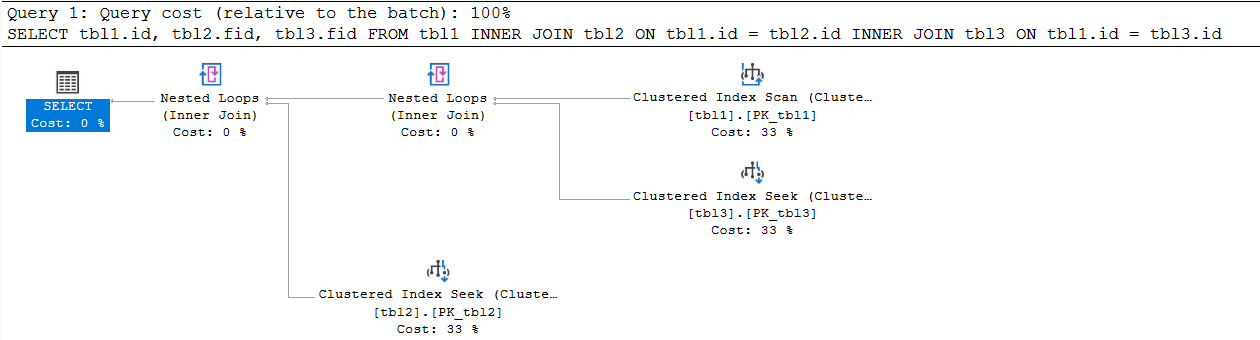
\includegraphics[width=\textwidth]{sample_plan2.png}
    \caption{Execution plan for sample query with no join hints}
\end{minipage}
\hfill
\end{figure}

The query plan can be used to create an equivalent eggplant query plan expression and the 
required input table metadata.  In a full end-to-end workflow this process would be automated.  
The following expression corresponds to the proceeding execution plan.

\begin{lstlisting}[language=bash,
    frame=single, numbers=left, numbersep=5pt, numberstyle=\tiny\color{mygray},]
(select (nestedLoopsJoin (nestedLoopsJoin (scan tbl1) (seek tbl3)) seek(tbl2)))
\end{lstlisting}

This expression and the associated metadata can be provided to eggplant to detect inefficiencies.
In this simple example, when eggplant processes the rewrite rules using the actual table cardinalities
it determines that \texttt{tbl1} and \texttt{tbl2} should use a hash join and that this intermediate result should
be joined with \texttt{tbl3} using a merge join.  All tables are accessed using a scan.  The subsequent sections 
will provide details on how these rewrite rules and cost functions are implemented.

\begin{lstlisting}[language=bash,
    frame=single, numbers=left, numbersep=5pt, numberstyle=\tiny\color{mygray},]
(select (mergeJoin (hashJoin (scan tbl1) scan(tbl2)) scan(tbl3)))
\end{lstlisting}

This query plan expression corresponds to the following T-SQL query.  Note the addition of query plan hints to force 
particular join algorithms and access methods.

\begin{lstlisting}[language=bash,
    frame=single, numbers=left, numbersep=5pt, numberstyle=\tiny\color{mygray},]
SELECT tbl1.id, tbl2.fid, tbl3.fid
FROM tbl1 INNER HASH JOIN tbl2 WITH (FORCESCAN)  ON tbl1.id = tbl2.fid
INNER MERGE JOIN tbl3 WITH (FORCESCAN) ON tbl1.id = tbl3.fid
\end{lstlisting}
    
This updated SQL statement with the added query hints will produce the following physical query execution plan.
For this example we assume that these new operations are preferable in this situation based on the
actual cardinalities of each of the tables.

\begin{figure}[H]
\centering
\begin{minipage}[b]{0.9\textwidth}
    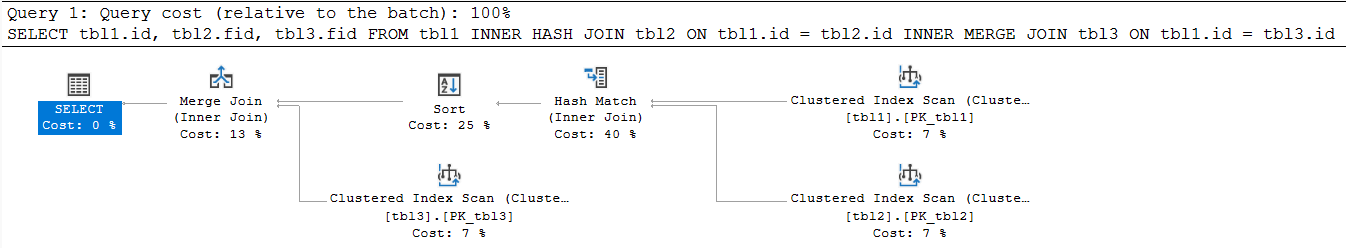
\includegraphics[width=\textwidth]{sample_plan1.png}
    \caption{Execution plan for sample query}
\end{minipage}
\hfill
\end{figure}

\section*{Egg Plan Transformer Design}
The Egg Plan Transformer (eggplant) is implemented as a Rust console application that uses the Egg expression 
rewriter library.  The application accepts a JSON input file that contains a query execution plan expression 
and metadata about the tables referenced in that expression.  Eggplant uses the facilities provided by the
Egg library to construct an e-graph and attach the query statistics metadata to e-nodes.  There is also a cost function
that evaluates various expression rewrite candidates to discover potentially beneficial transformations.
The lowest cost equivalent expression is printed as output.

It is important to consider the purpose of the eggplant tool when assessing its design.  Eggplant is a component
that is intended to be in the inner-core of a query performance tuning workflow, where the input is based on
query plans generated from commercial database systems.  These database systems have extensive optimization 
rules, data distribution metrics, and other specialized algorithms.  Eggplant is not trying to add new rules
that the DBMS is missing.  Instead its advantage is that the input metrics contain the actual metrics collected
from running the query, not based on estimates from data distribution statistics.  This allows eggplant to use the same rules 
as the DBMS but to produce a different, and potentially better plan, since differences between actual and estimated
cardinalities are a common source of suboptimal query plans.  The following diagram provides a high-level illustration
of eggplant inputs and outputs.

\begin{figure}[H]
\centering
\begin{minipage}[b]{1.0\textwidth}
    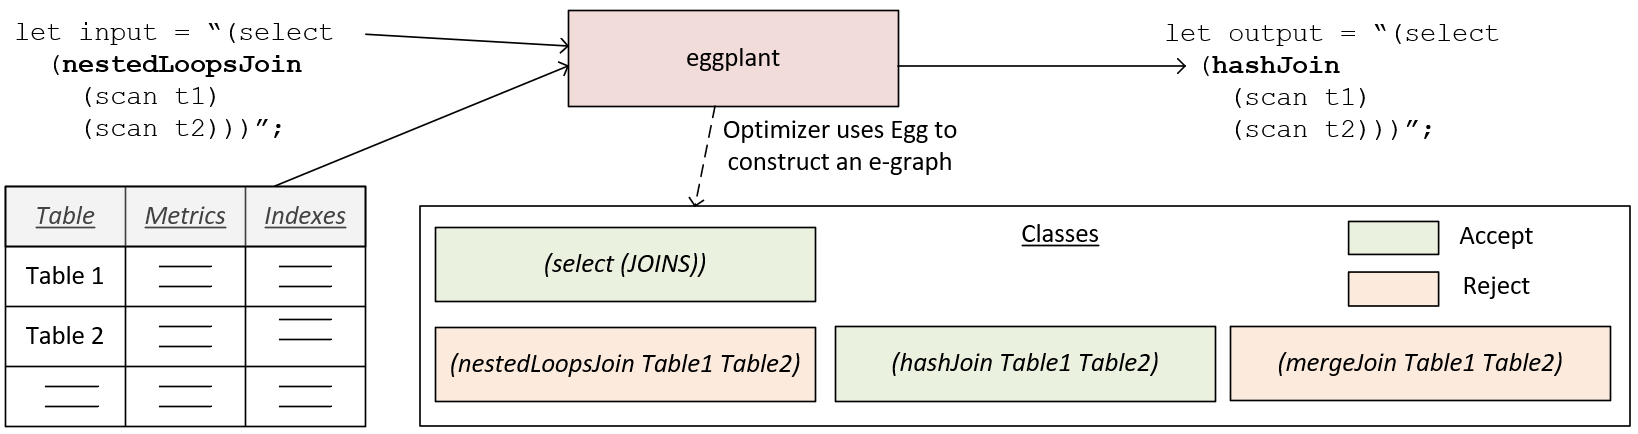
\includegraphics[width=\textwidth]{optimizer.png}
    \caption{Query execution plan post-processing with Egg-based optimizer}
\end{minipage}
\hfill
\end{figure}

Eggplant accepts an input JSON file that contains the query plan expression and related metadata.
Eggplant is a simple expression rewrite tool compared to an actual commercial query optimizer.
Therefore there is a limited collection of input metrics, such as actual cardinality, total rows in table,
index type, and whether the table is ordered.  The following example shows the specific input format.

\begin{lstlisting}[language=c++,
    frame=single, numbers=left, numbersep=5pt, numberstyle=\tiny\color{mygray},stringstyle=\ttfamily]
{
    // this is the input query plan expression that eggplant will try to transform
    "expression": "(select (mergeJoin (scan tbl1) (seek tbl2)))",
    // metadata about the tables in the expression for use in the cost function
    "tables": [
        {
            "name": "tbl1",          // name of the table in the expression
            "cardinality": 5,        // the actual cardinality of the table in the query
            "rows": 1000,            // the number of rows in the table
            "index": "primary",      // type of index (foreign or primary)
            "ordered": true          // whether the table will be processed in sorted order
        },
        {
            "name": "tbl2",
            "cardinality": 45,
            "rows": 50,
            "index": "foreign",
            "ordered": false
        }
    ]
}
\end{lstlisting}

\begin{figure}[H]
\centering
\begin{minipage}[b]{1.0\textwidth}
    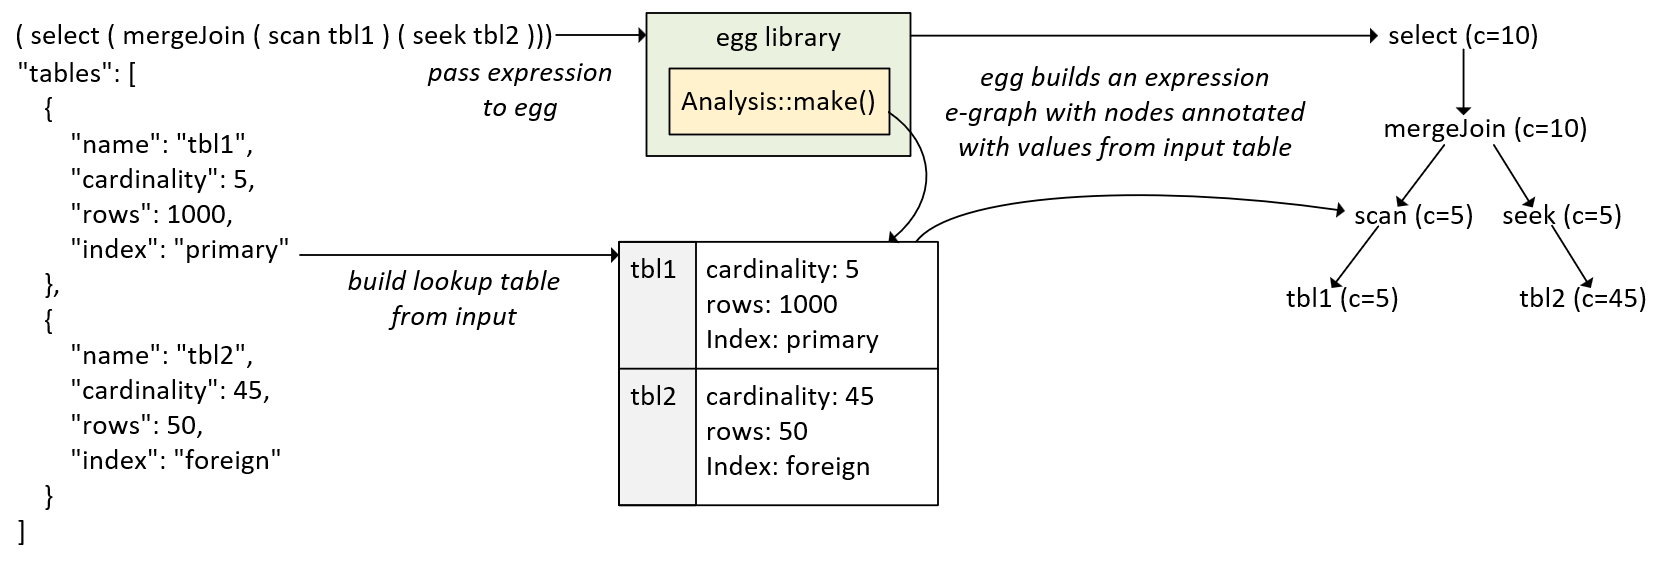
\includegraphics[width=\textwidth]{input_to_graph.png}
    \caption{Relationship of input metadata to expression e-graph}
\end{minipage}
\hfill
\end{figure}

The following figure illustrates how an example input expression could be transformed 
into an improved output expression.  First the input statement is transformed into an AST structure.
Then e-classes are created for potential rewrite optimizations.  In this example the e-classes
are for join operator and join order transformations.  The join operator is straightforward 
since the operators are functionally equivalent and can be interchanged without risk of creating
an invalid expression.  The join order is more complicated in that the rewrite rules need to 
ensure that the transformations are still valid.  In this specific example \texttt{tbl1} can 
join with either \texttt{tbl2} or \texttt{tbl3}, but \texttt{tbl2} cannot join directly with 
\texttt{tbl3}.  After the e-graph rewrites are complete there is a new AST which can be traversed
to generate the output expression.

\begin{figure}[H]
\centering
\begin{minipage}[b]{0.9\textwidth}
    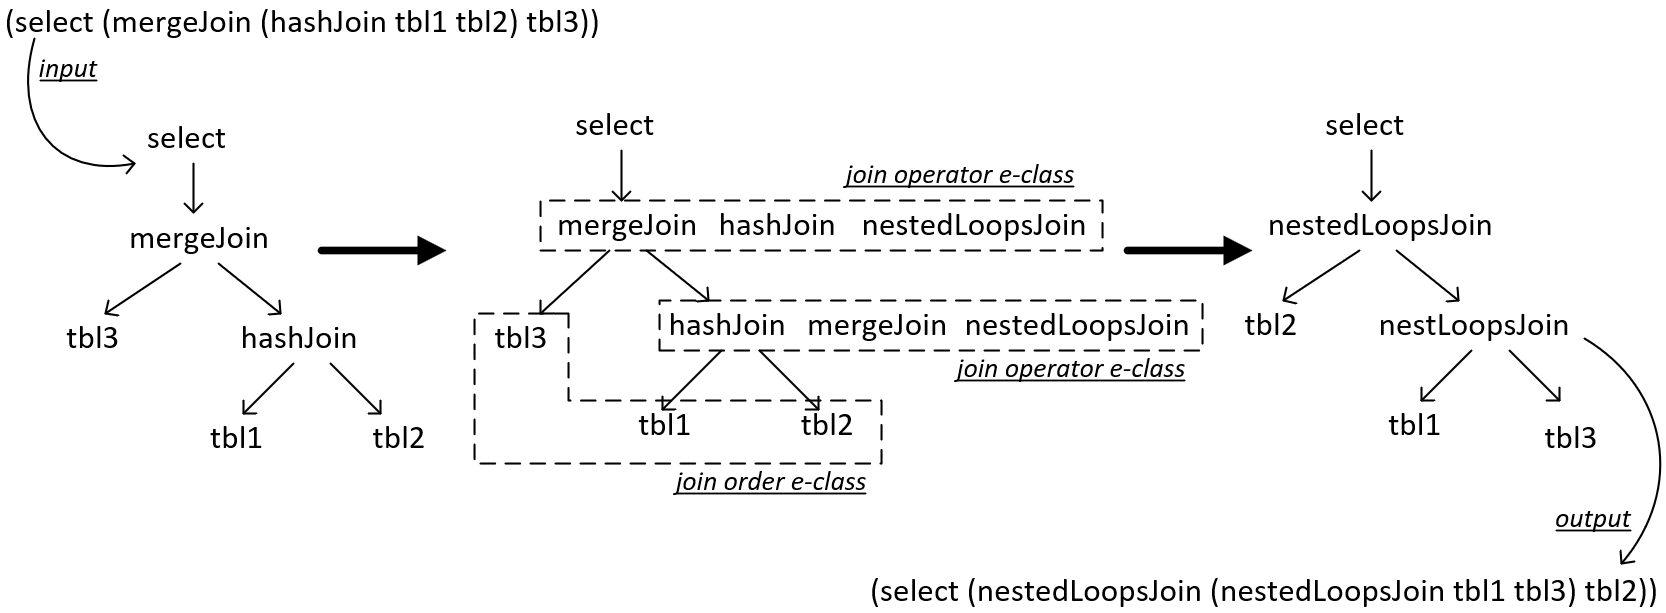
\includegraphics[width=\textwidth]{ast_transform.png}
    \caption{Transformation from input expression to output expression}
\end{minipage}
\hfill
\end{figure}

\section*{Eggplant Rules and Cost Functions}
Eggplant uses cost-based rewrite rules with the Egg equality saturation engine
to discover potential query plan improvements.  In each equivalent query plan expression the
eggplant cost function will apply context sensitive rules to determine the cost of each node.
The cost is generally a combination of the expected subtree cardinality combined with
various penalties to prevent undesirable expression rewrites.

The cost function will be given a set of actual cardinalities for each table.  It will use
these values to provide costs for join operation, join order, and access method.  Specifically,
whether to join using hash join, merge join, or nested loops join; whether to scan or seek each
table; and which order to use to join the tables.  There are common guidelines for when to perform
each of these optimizations to minimize intermediate result size and limit data I/O to process
a query.  \cite{West:2020}  

Eggplant supports a limited set of rewrite optimizations as a proof-of-concept to evaluate how 
well e-graph equality saturation works for cost-based query plan optimizations.  The specific set
of rules implemented include the following.

\begin{enumerate}
\item Expression tree reordering to create left-deep query plan trees
by moving join operators left of table inputs wherever possible.  Additionally, tables will be reordered
such that tables with primary keys will be moved left of tables with foreign keys.  This 
transformation simplifies the implementation of the join order rewrite rules.

\item Join order improvements to reduce the intermediate result set size for plans with multiple
join operators.  The basic idea is that if we have three tables combined in two joins, such
that $t_1 < t_2 < t_3$, then the expression would be changed from (join (join $t_1 t_3$) $t_2$) to 
(join (join $t_1 t_2$) $t_3$).

\item Access method selection for scanning or seeking the table storage.  The criteria is based on the 
proportion of the actual table cardinality with the number of rows in the table.  If 
$\operatorname{cardinality} / \operatorname{row\_count} >= 0.8$ (i.e. 80\% or more of the table)
is accessed then a scan is preferred, otherwise, if less than 20\% of the table is accessed then
a seek is preferred.

\item Join algorithm improvements to prefer either a hash join, merge join, or nested loops join.
This rule is overly simplistic compared to an actual query optimizer but it provides a 
good illustration of this cost-based rewrite technique.  The criteria for each join algorithm
is summarized in the below table.

\begin{tabular}{ | l | l | }
\hline
\textbf{Join Operator} & \textbf{Cost criteria} \\ \hline
Hash Join & One small table and one large table.  $t_1 <= 50$ and $t_2 > 1000$\\ \hline
Merge Join & No small tables or tables are ordered. $t_1 > 50$ and $t_2 > 50$ and $t_1 + t_2 > 1000$ \\ \hline
Nested Loops Join & Both tables are small. $t_1 + t_2 < 1000$  \\ \hline
\end{tabular}
\end{enumerate}

Determining the desired join order is challenging using the semantics of the Egg cost function methods.  
Consider the sample of potential arrangements of join operations and tables for the
case of two operators and three tables.  The position of the nodes in the tree is significant to 
the Egg rewrite engine.  There are 144 distinct arrangements of hash join, merge join, and nested loops
join with three tables.  Two considerations that arise while using these e-graphs are (1) how to write 
a minimal set of rewrite rules that will analyze all these expression tree configurations and (2) 
how to assign unique costs to each of the configurations when we only evaluate a single e-node
and its direct descendants at a time in the cost function.

\begin{figure}[H]
\centering
\begin{minipage}[b]{1.0\textwidth}
    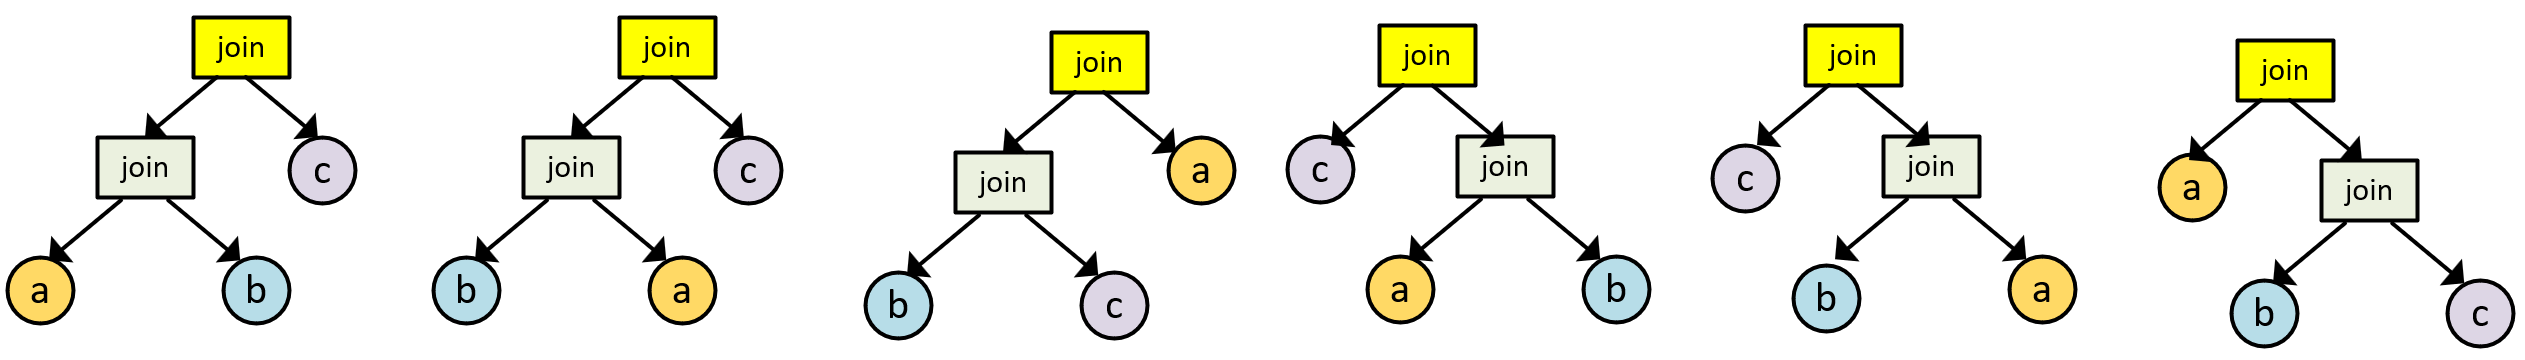
\includegraphics[width=\textwidth]{join_order.png}
    \caption{Join order table and algorithm combinations}
\end{minipage}
\hfill
\end{figure}

The cost functions use penalties to force preferred expression tree arrangements.  The penalties are arbitrary 
large numbers that can be assigned to nodes in order to exclude that expression from further consideration.
If the e-graph can be fully saturated then it is guaranteed that the alternate expression configurations that
are not penalized will be visited.  The below example illustrates how this process works for determining join 
order by moving smaller tables lower, and pushing joins and indexes left.  Specifically, cardinalities higher 
in the tree are scaled to 110\% cost and out of position primary key (PK) nodes are assigned a 100 cost 
penalty in this example.

\begin{figure}[H]
\centering
\begin{minipage}[b]{0.85\textwidth}
    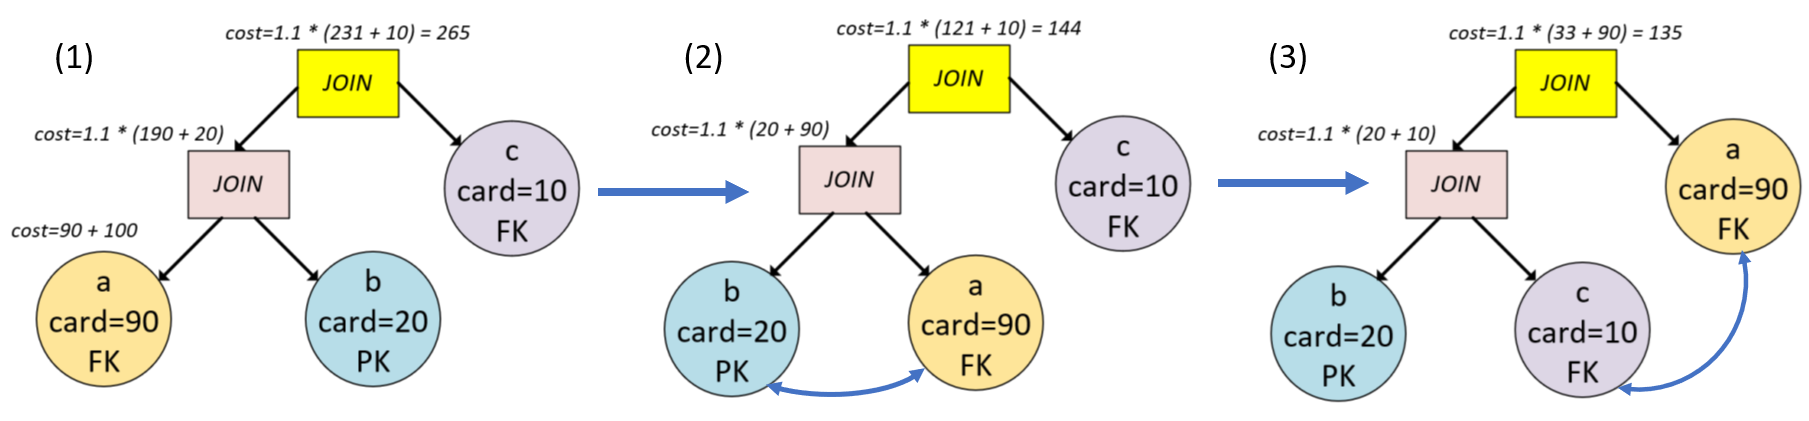
\includegraphics[width=\textwidth]{join_cost.png}
    \caption{Join order costing with penalties}
\end{minipage}
\hfill
\end{figure}

The following rewrite rules implement transformations for join order,
join algorithm, access method, and expression tree shape.  The rules only address a small subset of 
constructs that are possible with ANSI SQL statements.  Note that the access method and join ordering
rules are only defined for the hashJoin algorithms since Egg will convert other join algorithms to 
hashJoin during saturation, and then convert back to the preferred join method in the final expression.

\noindent \begin{tabular}{ | l | l | }
\hline
\textbf{Name} & \textbf{Type}  \\ \hline
idx-left & (hashJoin a b) $\rightarrow$ (hashJoin b a)  \\ \hline
order-right & (hashJoin (hashJoin a b) c) $\rightarrow$ (hashJoin (hashJoin a c) b)  \\ \hline
scan-seek & (hashJoin (scan a) b) $\rightarrow$ (hashJoin (seek a) b)  \\ \hline
seek-scan & (hashJoin (seek a) b) $\rightarrow$ (hashJoin (scan a) b)  \\ \hline
hash-join-merge-join & (hashJoin a b) $\rightarrow$ (mergeJoin a b)  \\ \hline
hash-join-nested-loops-join & (hashJoin a b) $\rightarrow$ (nestedLoopsJoin a b) \\ \hline
merge-join-hash-join & (mergeJoin a b) $\rightarrow$ (hashJoin a b)  \\ \hline
merge-join-nested-loops-join & (mergeJoin a b) $\rightarrow$ (nestedLoopsJoin a b) \\ \hline
nested-loops-join-merge-join & (nestedLoopsJoin a b) $\rightarrow$ (mergeJoin a b)  \\ \hline
nested-loops-join-hash-join & (nestedLoopsJoin a b) $\rightarrow$ (hashJoin a b) \\ \hline
\end{tabular}

The following code snippet is the eggplant hash join cost function implementation.  The concept
is that the join e-node will be able to access its child e-nodes that contain metrics
about the relation, such as cardinality, row count, etc.  These metrics will be compared with
rules for each operator to assign a penalty to each e-node.  The penalty is used as a signal the 
e-graph extraction algorithm to exclude the expression rewrites that are undesirable.

\begin{lstlisting}[language=C++,
    frame=single, numbers=left, numbersep=5pt, numberstyle=\tiny\color{mygray},stringstyle=\ttfamily]
// get the costs for the join operations according to join preference rules
fn get_hash_join_cost(egraph: &EPlanGraph, table1_id: &Id, table2_id: &Id) -> usize {
    let mut rank: usize = 800000;
    let t1_data = &egraph[*table1_id].data;             // get the e-node data object
    let t2_data = &egraph[*table2_id].data;
    let t1_cardinality = t1_data.cardinality;           // get cardinalities from data
    let t2_cardinality = t2_data.cardinality;
    if (t1_cardinality <= 50 || t2_cardinality <= 50)   // check if either table is small 
            && t1_cardinality + t2_cardinality > 1000 { // but that both tables together 
        rank = 2;                                       // aren't small
    }
    if t1_data.index.is_some() {                          // add penalty for foreign key 
        if t1_data.index.as_ref().unwrap() != "primary" { // on left node to force that 
            rank += 20000;                                // node to move right
        } else {
            rank += 10000;
        }
    }
    if t1_data.ordered && t2_data.ordered {    // if both tables are ordered than
        rank += 5000;                          // add penalty, this disqualifies
    }                                          // hash join and prefers merge join
    rank + t1_data.penalty + t2_data.penalty   // return join penalty plus child penalties 
}
\end{lstlisting}

The complete source code for the eggplant application can be reviewed at 


\noindent \href{https://github.com/kburtram/eggplant/blob/main/src/main.rs}{https://github.com/kburtram/eggplant/blob/main/src/main.rs}.

\section*{Project Results}
This project consists of the background design documented above and the implementation of the eggplant 
query plan expression optimizer.  The evaluation of this system is first based on whether the Egg e-graphs
are successfully configured to perform the desired rewrites with targeted plan expressions and table metrics.
The next evaluation is how well the optimizations reduce the expected size of intermediate results sets
from join order changes.  The following examples illustrate each of the rewrite rules with sample input metrics.

\textbf{Join algorithm and access method rewrites} Consider the following expression \textit{(select (mergeJoin (scan tbl1) (seek tbl2)))}
that joins two tables that are accessed with scan and seek methods.  Given the following three sets of metadata eggplant
will rewrite to hashJoin, nestedLoopsJoin and mergeJoin.  These examples demonstrate that in these simple cases the
rewrites are making the intended transformations based on the cost function rules.

\begin{lstlisting}[language=bash,
    frame=single, numbers=left, numbersep=5pt, numberstyle=\tiny\color{mygray},stringstyle=\ttfamily]
# Given the below table metrics
tbl1 -> cardinality:  5, rows: 1000, index: primary, ordered: true
tbl2 -> cardinality: 45, rows:   50, index: foreign, ordered: false
# Eggplant will rewrite to use nestedLoopsJoin and alternate scan/seek access methods
# Nested loops join is preferable when both tables are small
input       (select (mergeJoin (scan tbl1) (seek tbl2)))
output      (select (nestedLoopsJoin (seek tbl1) (scan tbl2)))

# Given the below table metrics
tbl1 -> cardinality: 3000, rows: 5000, index: primary, ordered: true
tbl2 -> cardinality:   20, rows: 1000, index: foreign, ordered: false
# Eggplant will rewrite to use hashJoin and alternate scan/seek access methods
# Hash join is preferred when one table is small and one is large
input       (select (mergeJoin (scan tbl1) (scan tbl2)))
output      (select (hashJoin (scan tbl1) (seek tbl2)))

# Given the below table metrics
tbl1 -> cardinality: 3000, rows: 5000, index: primary, ordered: true
tbl2 -> cardinality: 2000, rows: 5000, index: foreign, ordered: true
# Eggplant will not find any optimization opportunities
# Merge join is preferred when both tables are large and ordered
input       (select (mergeJoin (scan tbl1) (scan tbl2)))
output      (select (mergeJoin (scan tbl1) (scan tbl2)))
\end{lstlisting}

\textbf{Join ordering and parameter ordering rewrites} The rewrite rules implement basic
join table reordering and parameter reordering.  The parameter reordering will
move child join operator e-nodes left of child table e-nodes.  This has the effect of creating a left-deep
join tree.  The parameter reordering will also move the table accessed through its primary key
left of tables accessed through a foreign key.  This is to simplify the implementation of the 
join ordering rules while maintaining expression equivalency.  Specifically, the rules assume
when three tables are joined, one will have a primary key and the other two will have foreign keys.
In this case the tables with the foreign keys can be exchanged but the primary key table cannot 
be exchanged with a foreign key table without creating a non-equivalent query plan.  This assumption
limits the subset of SQL statements that can be processed with these rewrite rules, as there are
other valid ways to join three tables, such as using a different key for each of the join operations.

\begin{lstlisting}[language=bash,
    frame=single, numbers=left, numbersep=5pt, numberstyle=\tiny\color{mygray},stringstyle=\ttfamily]
# Given the below table metrics
tbl1 -> cardinality: 3000, rows: 4000, index: primary, ordered: true
tbl2 -> cardinality: 2000, rows: 4000, index: foreign, ordered: false
tbl3 -> cardinality: 1500, rows: 2000, index: foreign, ordered: false

# Eggplant will rewrite to move joins left to create a left-deep plan, and swaps 
# tbl2 and tbl3 in deepest join based on table size to minimize intermediate results size
input       (select (nestedLoopsJoin (scan tbl3) (mergeJoin (scan tbl1) (scan tbl2))))
output      (select (mergeJoin (mergeJoin (scan tbl1) (scan tbl3)) (scan tbl2)))
\end{lstlisting}

\textbf{Bringing it all together} These rules can be combined into arbitrarily complex expressions
and Egg will apply e-graph saturation to iteratively improve the expression.  The following example
is a more complete query plan expression that demonstrates how these rules work together
to create significantly transformed equivalent expressions that have a lower cost function.

\begin{lstlisting}[language=bash,
    frame=single, numbers=left, numbersep=5pt, numberstyle=\tiny\color{mygray},stringstyle=\ttfamily]
# Given the below table metrics
tbl1 -> cardinality: 3000, rows: 4000, index: primary, ordered: true
tbl2 -> cardinality: 2000, rows: 3000, index: foreign, ordered: false
tbl3 -> cardinality:   40, rows: 1000, index: foreign, ordered: false
tbl4 -> cardinality:  200, rows: 1000, index: foreign, ordered: false
tbl5 -> cardinality:  200, rows: 1000, index: foreign, ordered: false

# Eggplant will rewrite the input statement significantly applying all the rewrite rules, 
# including join order, join algorithm, expression tree shape, and access method
input        (select(
                nestedLoopsJoin(
                    nestedLoopsJoin(
                        mergeJoin (scan tbl1) (scan tbl2)) 
                        (scan tbl3)) 
                    (hashJoin (scan tbl4) (scan tbl5))))
output       (select(
                mergeJoin(
                    mergeJoin(
                        mergeJoin(
                            hashJoin (scan tbl1) (seek tbl3)) 
                            (scan tbl5)) 
                        (scan tbl4)) 
                    (scan tbl2)))
\end{lstlisting}

This example demonstrates the flexibility in the eggplant implementation to make broad improvements
to query execution plans while only applying rules at a single e-node at a time.  This is possible because Egg
enumerates through all the permutations of different expression configurations allowing costs
and penalties to propagate through the expression tree.  This example expression makes over 5000 calls into
cost functions as it applies the rewrite rules to generate candidate expressions.  The effect of the cost-based
rewrite rules can be observed from comparing the input metrics above and the expression tree transformation below.
The final expression tree is left-deep, smaller tables are moved down except the primary key table remains at the bottom, 
hash joins and merge joins are used based on expected table sizes, and access methods are selected 
based on the cardinality-to-row count ratio.  This illustrates that eggplant is performing the 
expected optimizations consistently even with more complex query plan expressions.

\begin{figure}[H]
\centering
\begin{minipage}[b]{1.0\textwidth}
    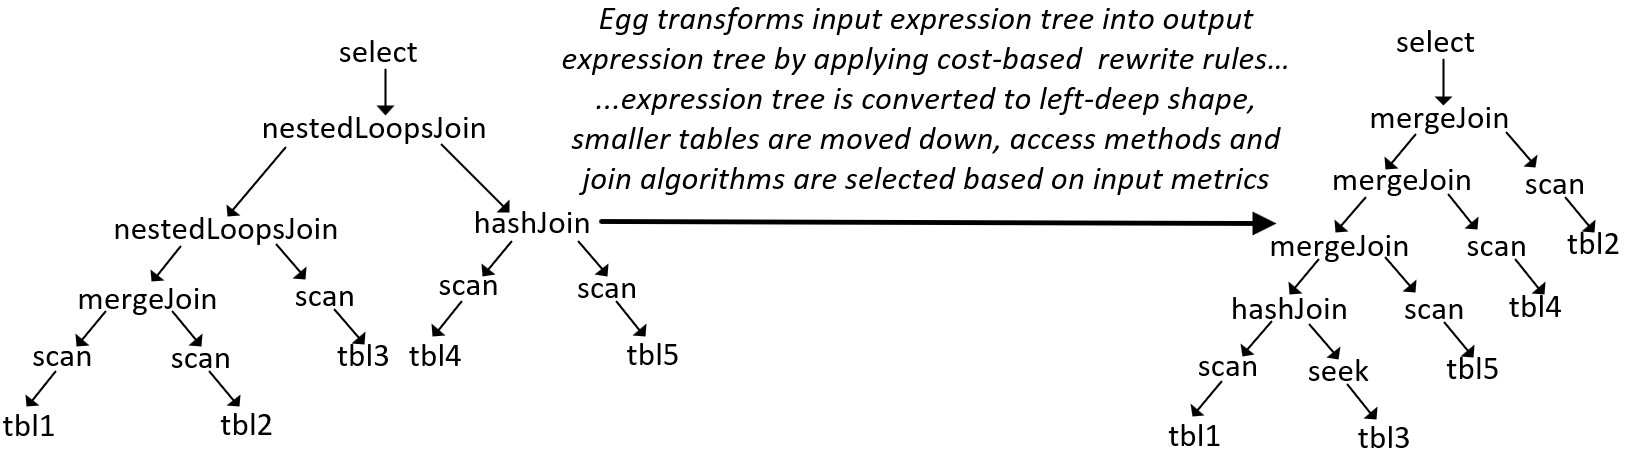
\includegraphics[width=\textwidth]{complex-transform.png}
    \caption{Expression tree transformation for complex query plan expression}
\end{minipage}
\hfill
\end{figure}

The following experiment was used to assess the effectiveness of the join order optimizations.  Random expressions and 
table metrics were generated with table sizes from 2 through 15.  These were run through eggplant and the average
intermediate result size was collected.  Intermediate result size was determined by summing the cardinality of the
join operator e-nodes in the e-graph.  Eggplant was able to find significant improvements in expressions with at
least 3 tables, with improvements leveling off between 40\% and 50\% after 5 tables.  The first chart shows the
total intermediate results sizes and the second chart shows the cardinality and penalty improvement percentages.  
The Python notebook used to run this experiments is available at
\href{https://github.com/kburtram/eggplant/blob/main/analysis/analysis.ipynb}{https://github.com/kburtram/eggplant/blob/main/analysis/analysis.ipynb}

\begin{figure}[H]
\centering
\begin{minipage}[b]{0.65\textwidth}
    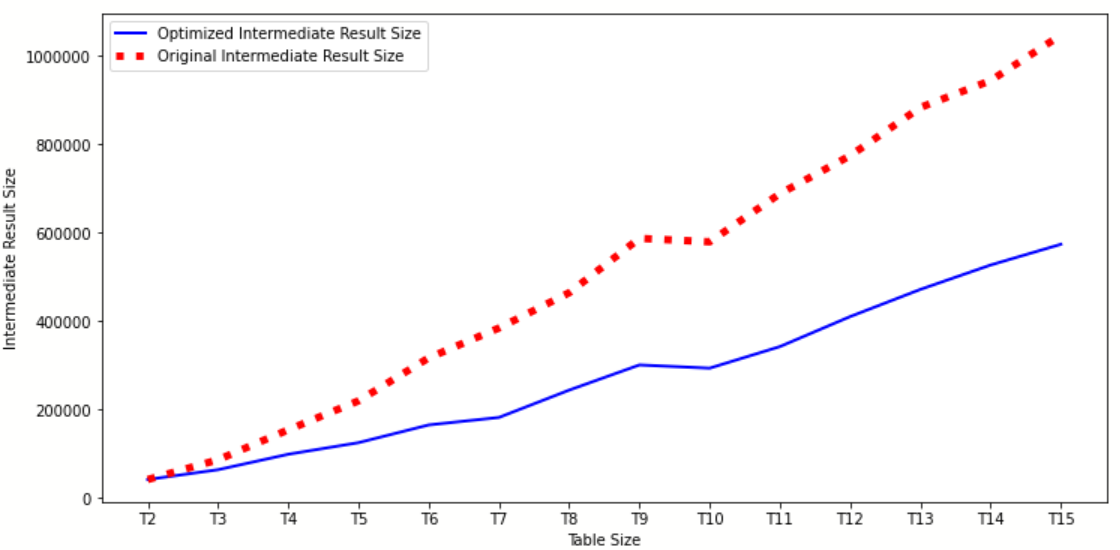
\includegraphics[width=\textwidth]{result_size.png}
    \caption{Intermediate table results size by table count}
\end{minipage}
\hfill
\end{figure}

Note that as expected the cardinality and penalty improvements are highly correlated since a significant portion of the
penalty is computed based on cardinality.  The improvements were consistent even as the table count was increased to 50, 
indicating that with full saturation global optimizations are possible.

\begin{figure}[H]
\centering
\begin{minipage}[b]{0.65\textwidth}
    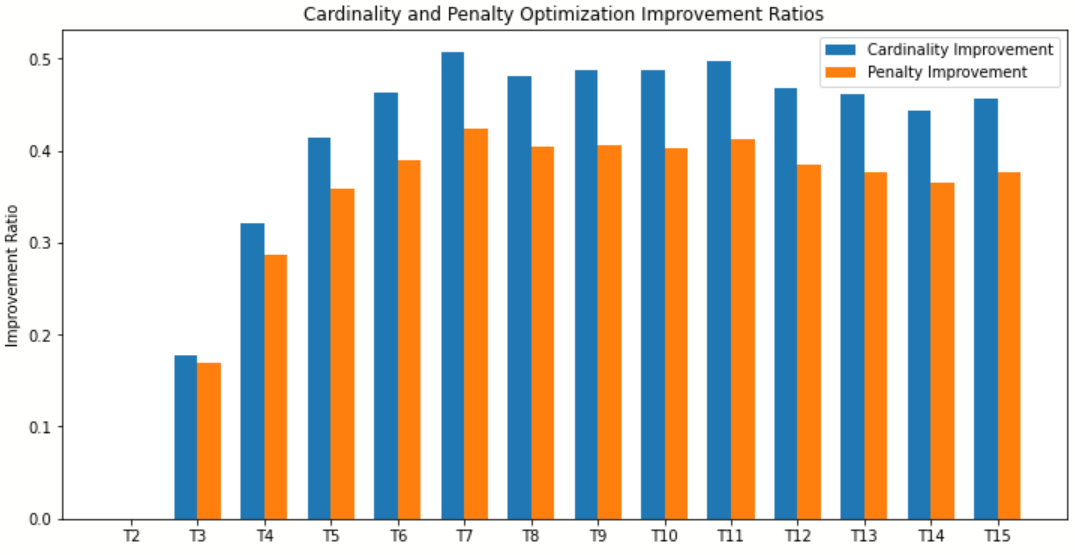
\includegraphics[width=\textwidth]{result_percent.png}
    \caption{Cardinality and penalty improvement by table count}
\end{minipage}
\hfill
\end{figure}

\section*{Conclusion}
The goal of this project was to investigate whether e-graph equality saturation techniques can be used as part of a
query performance tuning workflow to identify execution plan inefficiencies.  The details around executing SQL queries
to generate plans, converting plans to the query plan expression language, and generating query plan hints have
been omitted from this project.  The project has focused on defining a simple expression language for a subset of physical query plan
operators and defining cost-based rewrite rules to implement a small set of query plan optimizations.

The project successfully implemented the eggplant tool that can perform a limited set of query
plan expression rewrites based on input table metrics.  The project result is neutral in that the eggplant implementation 
is likely not the ideal mechanism for some of the query plan transformations.  Particularly the join ordering 
rules are relatively limited as only three tables are considered at a time, making global optimizations more
difficult.  Additionally, the model of using penalties to control the expression rewrites seems to have some limitations
when many rules are considered together.  The approach generally works since the expression that avoids all the penalties
will be selected with full saturation.  The eggplant implementation demonstrates complex parsing and rewriting techniques based on the Egg library.  
Eggplant's general approach could be extended to encompass a more complete set of rules to better improve the query performance tuning workflow. 

\begin{thebibliography}{100} % Bibliography 

\bibitem[Ben-Gan, 2015]{BenGan:2015}
Ben Gan, Itzik; Sarka, Dejan; Mechanic, Adam; Farlee, Kevin (2015)
\\\newblock \textit{T-SQL Querying}

\bibitem[Fritchey, 2014]{Fritchey:2014}
Fritchey, Grant (2014)
\\\newblock \textit{SQL Server Query Performance Tuning}

\bibitem[Korotkevitch, 2012]{Korotkevitch:2014}
Korotkevitch, Dmitri (2014)
\\\newblock \textit{Pro SQL Server Internals}

\bibitem[Wang, et al., 2020]{Wang:2020}
Wang, Yisu Remy ; Hutchison, Shana; Leang, Jonathan; Howe, Bill; Suciu, Dan (2020)
\\\newblock \textit{SPORES: Sum-Product Optimization via Relational Equality Saturation for Large Scale Linear Algebra}

\bibitem[West, et al., 2020]{West:2020}
West, Randolph; Zecharias, Melody; Assaft, William; Aelterman, Sven; et al. (2020)
\\\newblock \textit{SQL Server 2019 Administration}

\bibitem[Willsey, et al., 2020]{Willsey:2020}
Willsey, Max; Nandi, Chandrakana; Wang, Yisu Remy; Flatt, Oliver; et al. (2020)
\\\newblock \textit{egg: Fast and Extensible Equality Saturation}

\bibitem[Yang, et al., 2020]{Yang:2021}
Yang, Yichen; Phothilimthana, Phitchaya Mangpo; Wang, Yisu Remy  et al. (2021)
\\\newblock \textit{Equality Saturation for Tenor Graph Superoptimization}

\end{thebibliography}

\section*{Source Code and Artifacts}

\noindent eggplant GitHub - \href{https://github.com/kburtram/eggplant}{https://github.com/kburtram/eggplant}

\null

\noindent eggplant main source code - \noindent \href{https://github.com/kburtram/eggplant/blob/main/src/main.rs}{https://github.com/kburtram/eggplant/blob/main/src/main.rs}

\null

\noindent eggplant experiment notebook - \href{https://github.com/kburtram/eggplant/blob/main/analysis/analysis.ipynb}{https://github.com/kburtram/eggplant/blob/main/analysis/analysis.ipynb}

\null

\noindent Presentation slides - \href{https://github.com/kburtram/eggplant/raw/main/docs/kburtram-presentation.pptx}{https://github.com/kburtram/eggplant/raw/main/docs/kburtram-presentation.pptx}

\null

\noindent Final report - \href{https://github.com/kburtram/eggplant/blob/main/docs/karlburtram-report.pdf}{https://github.com/kburtram/eggplant/blob/main/docs/karlburtram-report.pdf}

\end{document}
